%%%%%%%%%%%%%%%%%%%%%%%%%%%%%%%%%%%%%%%%%
% Jacobs Landscape Poster
% LaTeX Template
% Version 1.1 (14/06/14)
%
% Created by:
% Computational Physics and Biophysics Group, Jacobs University
% https://teamwork.jacobs-university.de:8443/confluence/display/CoPandBiG/LaTeX+Poster
% 
% Further modified by:
% Nathaniel Johnston (nathaniel@njohnston.ca)
%
% This template has been downloaded from:
% http://www.LaTeXTemplates.com
%
% License:
% CC BY-NC-SA 3.0 (http://creativecommons.org/licenses/by-nc-sa/3.0/)
%
%%%%%%%%%%%%%%%%%%%%%%%%%%%%%%%%%%%%%%%%%

%----------------------------------------------------------------------------------------
%	PACKAGES AND OTHER DOCUMENT CONFIGURATIONS
%----------------------------------------------------------------------------------------

\documentclass[final, 14pt]{beamer}

\usepackage[scale=1.24]{beamerposter} % Use the beamerposter package for laying out the poster
\usetheme{confposter} % Use the confposter theme supplied with this template

\setbeamercolor{title}{fg=BrickRed}
\setbeamercolor{block title}{fg=cardinalred,bg=white} % Colors of the block titles
\setbeamercolor{block body}{fg=black,bg=white} % Colors of the body of blocks
\setbeamercolor{block alerted title}{fg=white,bg=cardinalred} % Colors of the highlighted block titles
\setbeamercolor{block alerted body}{fg=black,bg=cardinalred!10} % Colors of the body of highlighted blocks
% Many more colors are available for use in beamerthemeconfposter.sty

%-----------------------------------------------------------
% Define the column widths and overall poster size
% To set effective sepwid, onecolwid and twocolwid values, first choose how many columns you want and how much separation you want between columns
% In this template, the separation width chosen is 0.024 of the paper width and a 4-column layout
% onecolwid should therefore be (1-(# of columns+1)*sepwid)/# of columns e.g. (1-(4+1)*0.024)/4 = 0.22
% Set twocolwid to be (2*onecolwid)+sepwid = 0.464
% Set threecolwid to be (3*onecolwid)+2*sepwid = 0.708

\newlength{\sepwid}
\newlength{\onecolwid}
\newlength{\twocolwid}
\newlength{\threecolwid}
\setlength{\paperwidth}{48in} % A0 width: 46.8in
\setlength{\paperheight}{36in} % A0 height: 33.1in
\setlength{\sepwid}{0.024\paperwidth} % Separation width (white space) between columns
\setlength{\onecolwid}{0.22\paperwidth} % Width of one column
\setlength{\twocolwid}{0.464\paperwidth} % Width of two columns
\setlength{\threecolwid}{0.708\paperwidth} % Width of three columns
\setlength{\topmargin}{-0.5in} % Reduce the top margin size
%-----------------------------------------------------------

\usepackage{graphicx}  % Required for including images
\usepackage{booktabs} % Top and bottom rules for tables
%\renewcommand{\cite}{\citet}

%----------------------------------------------------------------------------------------
%	TITLE SECTION 
%----------------------------------------------------------------------------------------

\title{Warfarin Dosage with LinUCB and Supervised Learning} % Poster title

\author{Haojun Li} % Author(s)

\institute{Department of Computer Science, Stanford University} % Institution(s)
\addtobeamertemplate{headline}{} 
{
	\begin{tikzpicture}[remember picture,overlay] 
	\node [shift={(12 cm,-8cm)}] at (current page.north west) {
\includegraphics[height=10cm]{Stanford-Logo.png}}; 
	\end{tikzpicture} 
}
%----------------------------------------------------------------------------------------

\begin{document}

\addtobeamertemplate{block end}{}{\vspace*{2ex}} % White space under blocks
\addtobeamertemplate{block alerted end}{}{\vspace*{2ex}} % White space under highlighted (alert) blocks

\setlength{\belowcaptionskip}{2ex} % White space under figures
\setlength\belowdisplayshortskip{2ex} % White space under equations

\begin{frame}[t] % The whole poster is enclosed in one beamer frame

\begin{columns}[t] % The whole poster consists of three major columns, the second of which is split into two columns twice - the [t] option aligns each column's content to the top

\begin{column}{\sepwid}\end{column} % Empty spacer column

\begin{column}{\onecolwid} % The first column

%----------------------------------------------------------------------------------------
%	OBJECTIVES
%----------------------------------------------------------------------------------------

\begin{alertblock}{Abstract}

Predicting the correct dosage of Warfarin is a challenge. Most researchers estimate the correct dosage by first gathering data on the correct dosage and then eventually devise an algorithm for the correct dosage. \cite{international2009estimation} We experimented with the following methods
\begin{itemize}
	\item LinUCB with Disjoint models. Predicting the reward for each dosage category independently
	\item Supervised learning with linear models in a RL-fashion
\end{itemize}
We showed that both models are able to beat the Fixed Dose baseline and Clinical Dosage baseline in terms of regret, but unable to beat the Clinical Dosage baseline in terms of fraction of incorrect cases.

\end{alertblock}

%----------------------------------------------------------------------------------------
%	INTRODUCTION
%----------------------------------------------------------------------------------------

\begin{block}{Data and Features}
The data we were given contains patient features (such as age and height) as well as the actual Therapeutic Dose of Warfarin. The goal is to predict the correct dosage of Warfarin from these features using a linear model in a simulated setting where patients comes in one at a time.

One major assumption is that the actual dosage of Warfarin is linear to the features of the patients. In order to keep comparisons against the baselines fair, we will use the same set of features that Clinical Dosage baseline uses, which are \textbf{Race, Age in decades, Height (cm), Weight (kg), Carba- mazepine (Tegretol), Amiodarone (Cordarone), Pheny- toin (Dilantin), Rifampin or Rifampicin.} These are also the features used in computing the regret for each algorithm

\end{block}

%----------------------------------------------------------------------------------------

\end{column} % End of the first column

\begin{column}{\sepwid}\end{column} % Empty spacer column

\begin{column}{\twocolwid} % Begin a column which is two columns wide (column 2)

\begin{columns}[t,totalwidth=\twocolwid] % Split up the two columns wide column

\begin{column}{\onecolwid}\vspace{-.6in} % The first column within column 2 (column 2.1)

%----------------------------------------------------------------------------------------
%	MATERIALS
%----------------------------------------------------------------------------------------

\begin{block}{LinUCB $\alpha$ search}

The LinUCB algorithm with disjoint models is the same as referenced in the news recommendation paper \cite{li2010contextual}. However, the parameter $\alpha$ needs to be tuned to push the agent to explore less and exploit more due to the short time horizon (5528 patients)

\begin{figure}
	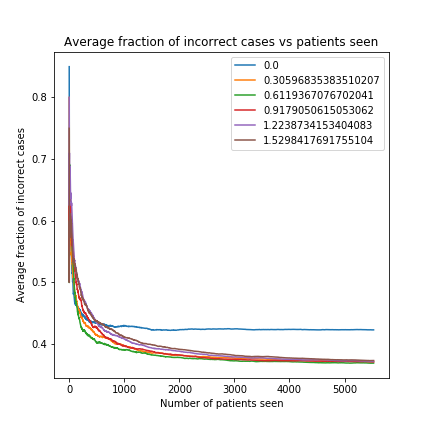
\includegraphics[width=\linewidth]{../plots/avg_frac_alphas.png}
\end{figure}


\end{block}
%\begin{figure}
%	\centering
%	\includegraphics[width=\linewidth]{../plots/cnn-rnn-model}
%	\caption{Attended CNN Encoder + RNN}
%	\label{fig:cnn-rnn-model}
%\end{figure}

%----------------------------------------------------------------------------------------

\end{column} % End of column 2.1

\begin{column}{\onecolwid}\vspace{-.6in} % The second column within column 2 (column 2.2)

%----------------------------------------------------------------------------------------
%	METHODS
%----------------------------------------------------------------------------------------

\begin{block}{Results and Discussion}
We evaluated all the models using 20 different trials. For LinUCB, we used $\alpha = 0.612$ and for Supervised Learning approach we used a batch size of 50. Results are in table \ref{results}

\vspace{.5in}

\begin{table}[h]
	\label{results}
	\centering
	\begin{tabular}{ccc}
					\toprule
					Method          & Avg Total Regret & Avg Fraction    \\
					\midrule
					Fixed Dose      & 61.53            & 0.3882          \\
					Clinical Dosing & 54.227           & \textbf{0.3572} \\
					LinUCB          & 51.45            & 0.3692          \\
					Logistic        & \textbf{33.49}   & 0.3598    	\\
					\bottomrule
	\end{tabular}
	\caption{Results from experiments}
\end{table}

LinUCB and Supervised Learning does better in terms of Fixed Dose and Clinical Dosing Algorithms in terms of regret but not able to achieve better average fraction of incorrect cases due to the fact that it has an initial exploration period. 

The plot below shows that LinUCB does explore longer than supervised learning before finally arriving at a good set of parameters and quickly catching up to the other models, while  Clinical Dosing Algorithm makes correct predictions right from the beginning

\end{block}

%----------------------------------------------------------------------------------------

\end{column} % End of column 2.2

\end{columns} % End of the split of column 2 - any content after this will now take up 2 columns width

%----------------------------------------------------------------------------------------
%	IMPORTANT RESULT
%----------------------------------------------------------------------------------------

%----------------------------------------------------------------------------------------

\begin{columns}[t,totalwidth=\twocolwid] % Split up the two columns wide column again

\begin{column}{\onecolwid} % The first column within column 2 (column 2.1)

%----------------------------------------------------------------------------------------
%	MATHEMATICAL SECTION
%----------------------------------------------------------------------------------------

\begin{block}{Supervised Learning Approach}
In a supervised setting, the agent will see 50 patients at a time and train a model on all the data gathered as well as their true dosage. Then at each step, the agent will predict which dosage category should be used. Table below shows 2 different model classes when fitted and evaluated on the entire dataset (thus an upper limit of performance)

\vspace{.5in}
	
\begin{table}[h]
	\label{results2}
	\centering
	\begin{tabular}{ccc}
					\toprule
					Model Class         & Optimal Regret & Optimal Fraction\\
					\midrule
					Logistic & \textbf{30.93}          & \textbf{0.3538}  \\
					SVM                 & 61.53          & 0.3882 \\
					\bottomrule
	\end{tabular}
	\caption{Results from different model classes}
\end{table}

SVM does significantly worse than Logistic Regression since there is linear structure in the dataset.

\end{block}

%----------------------------------------------------------------------------------------

\end{column} % End of column 2.1

\begin{column}{\onecolwid} % The second column within column 2 (column 2.2)

%----------------------------------------------------------------------------------------
%	RESULTS
%----------------------------------------------------------------------------------------

\begin{block}{Plots}

\begin{figure}
	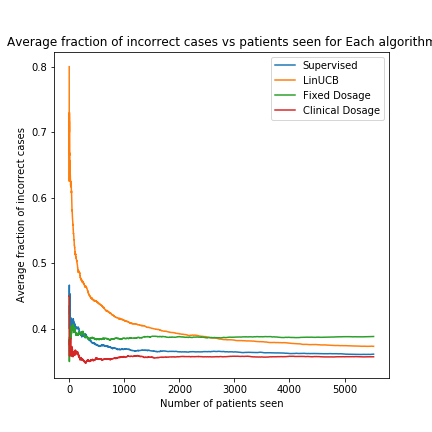
\includegraphics[width=\linewidth]{../plots/avg_frac_algos.png}
\end{figure}


\end{block}

%----------------------------------------------------------------------------------------

\end{column} % End of column 2.2

\end{columns} % End of the split of column 2

\end{column} % End of the second column

\begin{column}{\sepwid}\end{column} % Empty spacer column

\begin{column}{\onecolwid} % The third column

%----------------------------------------------------------------------------------------
%	CONCLUSION
%----------------------------------------------------------------------------------------

\begin{block}{Conclusion}

\begin{itemize}
	\item LinUCB with a lower $\alpha$ value is able to achieve lower regret than both baselines. This low $\alpha$ balances exploration and exploitation, and attempts to arrive at a sub-optimal parameters quicker due to the short horizon
	\item Supervised Learning method performed significantly better than other methods, but due to its exploration period it is unable to outperform Clinical Dosing Algorithm in terms of average fraction of incorrect cases.
\end{itemize}
\end{block}

%----------------------------------------------------------------------------------------
%	ADDITIONAL INFORMATION
%----------------------------------------------------------------------------------------

\begin{block}{Future Works}

A lot still need to be done if I have more time
\begin{itemize}
\item Explore different Bandit algorithms with better bounds.
\item Explore more $\alpha$ values for a better balance in exploration/exploitation
\end{itemize}

\end{block}

%----------------------------------------------------------------------------------------
%	REFERENCES
%----------------------------------------------------------------------------------------

\begin{block}{References}

\nocite{*} % Insert publications even if they are not cited in the poster
\small{\bibliographystyle{unsrt}
\bibliography{ref}\vspace{0.5in}}

\end{block}

%----------------------------------------------------------------------------------------
%	ACKNOWLEDGEMENTS
%----------------------------------------------------------------------------------------

\setbeamercolor{block title}{fg=red,bg=white} % Change the block title color

%----------------------------------------------------------------------------------------
%	CONTACT INFORMATION
%----------------------------------------------------------------------------------------

\setbeamercolor{block alerted title}{fg=black,bg=norange} % Change the alert block title colors
\setbeamercolor{block alerted body}{fg=black,bg=white} % Change the alert block body colors

%----------------------------------------------------------------------------------------

\end{column} % End of the third column

\end{columns} % End of all the columns in the poster

\end{frame} % End of the enclosing frame

\end{document}
